\documentclass[11pt]{ctexrep}
\usepackage{amsmath,amssymb,mathtools,amsthm} % 数学相关宏包
\usepackage{geometry,hyperref}                % 页面布局+超链接
\usepackage{graphicx}                         % 插图宏包
\usepackage{tcolorbox}                         % 定理框宏包
\tcbuselibrary{theorems,skins}

%% 页面设置
\geometry{margin=1in}
\renewcommand\thesection{\arabic{section}}
\hypersetup{colorlinks=true,linkcolor=blue,anchorcolor=blue,citecolor=blue}

%% tcolorbox样式（仅用于核心定义/模型，保持原样式）
\tcbset{
    mystyle/.style={
        colback=blue!5,colframe=blue!75!black,
        fonttitle=\bfseries,boxrule=0.8pt,
        left=10pt,right=10pt,top=8pt,bottom=8pt
    }
}
%% 带编号的定义环境（tcolorbox版）
\newtcbtheorem[number within=section]{defn}{定义}{mystyle}{def}
% 普通定理/备注环境
\newtheorem{remark}{注}[section]

%% 标题与作者
\title{后向可达集\\Backward Reachable Set (BRS)}
\author{武 朝康}
\date{\today}

%% 正文
\begin{document}
\maketitle
%\tableofcontents

\section{引言}
在动力学系统中，后向可达集 (Backward Reachable Set, BRS) 描述的是所有初始状态的集合，系统从这一集合出发，能够在未来的特定时间范围内到达给定的最终状态目标集。

在控制系统的分析中，存在两类不同的问题：一类是轨迹与控制律设计问题，核心关注系统\emph{如何}被控制，这类问题通常追求最优性或特定性能指标；另一类是安全性与可达性问题，核心关注系统\emph{能否}达到某个集合，这类问题仅关注控制策略的存在性。

在飞行器安全分析、失效后能力评估等实际工程问题中，我们往往并不关心控制输入的具体形式，而更关心是否\emph{存在}某种控制策略，使系统能够在给定时间内进入安全区域。后向可达集正是用于回答这一类“能不能”的存在性问题，近年来其在安全验证、飞行器失效安全分析与鲁棒控制中被频繁使用。

然而，在初次接触BRS时，其时间方向、Hamiltonian 中的极值运算，以及值函数 $\phi$ 的物理与语义含义，往往给学习者带来困惑。本文尝试从研究者的视角，对后向可达集的核心概念、Hamilton---Jacobi 方程的构造逻辑，以及若干关键但常被忽略的细节进行一次系统性的理解整理。

\section{后向可达集的数学定义}
研究后向可达集的前提是定义非线性控制系统的动力学模型，本文考虑一般的非线性控制系统形式，并要求系统的向量场满足Lipschitz连续条件——这一条件是保证系统解的存在与唯一性的关键，也是后续分析的基础。

\subsection{非线性控制系统动力学}
本文研究的非线性控制系统核心模型如下，其为后向可达集分析的基础形式：
\begin{tcolorbox}[mystyle,title={模型定义}]
考虑非线性控制系统：
\begin{equation}\label{eq:dyn}
\dot{\mathbf{x}}(\tau) = f(\mathbf{x}(\tau), \mathbf{u}(\tau))
\end{equation}
其中：
	\begin{itemize}
		\item $\tau \in [t,0]$为时间域，$t<0$为初始时刻，$0$为目标时刻。
		\item  $\mathbf{x}(\tau) \in \mathbb{R}^n$ 为$n$维系统状态向量；
		\item $\mathbf{u}(\tau) \in \mathcal{U} \subset \mathbb{R}^m$ 为$m$维容许控制输入，$\mathcal{U}$为控制输入的可行域；
	\end{itemize}
\end{tcolorbox}

为保证上述系统解的存在性与唯一性，要求向量场 $f(\mathbf{x},\mathbf{u},t): \mathbb{R}^n \times \mathbb{R}^m \times \mathbb{R} \to \mathbb{R}^n$ 满足Lipschitz连续条件，其严格数学定义如下：

\begin{defn}{Lipschitz 连续}{lipschitz}
设 $(X, \|\cdot\|)$ 与 $(Y,\|\cdot\|)$ 为赋范空间，函数 $f:D\subset X\to Y$ 在非空子集$D$上称为Lipschitz 连续，若存在常数 $L\ge0$，使得对任意 $x,y\in D$ 有
\[
\|f(x)-f(y)\|\le L\|x-y\|.
\]
满足上述不等式的最小非负常数 $L$ 称为函数 $f$ 在集合$D$上的Lipschitz 常数。
\end{defn}

\subsection{后向可达集的严格定义}
记 $t=0$ 时刻系统的目标集为 $\mathcal{T} \subset \mathbb{R}^n$，结合上述非线性控制系统模型，$t$ \textbf{时刻的后向可达集}被严格定义为：
\[
\mathcal{R}_t(\mathcal{T}) = \left\{ \mathbf{x}(t) \in \mathbb{R}^n \bigg| \exists \mathbf{u}(\cdot) \in \mathcal{U}, \text{ 使得 } \mathbf{x}(0) \in \mathcal{T} \right\}
\]
其核心语义为：$\mathcal{R}_t(\mathcal{T})$是 $t$ 时刻状态的一个集合，从该集合中的任意状态出发，\textbf{存在}可行的控制输入 $\mathbf{u}(\cdot) \in \mathcal{U}$，使系统在时间演化至 $0$ 时刻时，状态能进入目标集 $\mathcal{T}$。

特别地，当取初始时刻 $t = -T$（$T>0$为正的时间长度）时，$\mathcal{R}_{-T}(\mathcal{T})$ 表示更直观的物理含义：从该集合出发，存在可行控制输入使系统在$T$个单位时间后准确到达目标集 $\mathcal{T}$ 的所有初始状态。

\vspace{1.5ex}
为了更方便地刻画后向可达集这一集合特征，引入隐式值函数 $\phi(\mathbf{x},t): \mathbb{R}^n \times \mathbb{R} \to \mathbb{R}$，该函数与后向可达集的等价关系为：
\[
\phi(\mathbf{x},t) \le 0 \quad \Longleftrightarrow \quad \mathbf{x} \in \mathcal{R}_t(\mathcal{T})
\]
即状态$\mathbf{x}$在$t$时刻属于后向可达集，当且仅当值函数在该状态-时间点的取值小于等于0。

如图 \ref{fig:levelSetFunctionandTargetSet}，一个二维状态空间的值函数 $\phi(x,y,0)$ 的截面 $\phi=0$ 对应的截面曲线即为目标集 $\mathcal{T}$ 的边界（$t=0$ 时刻）。
\vspace{1.5ex}
\begin{figure}[htbp]
    \centering
    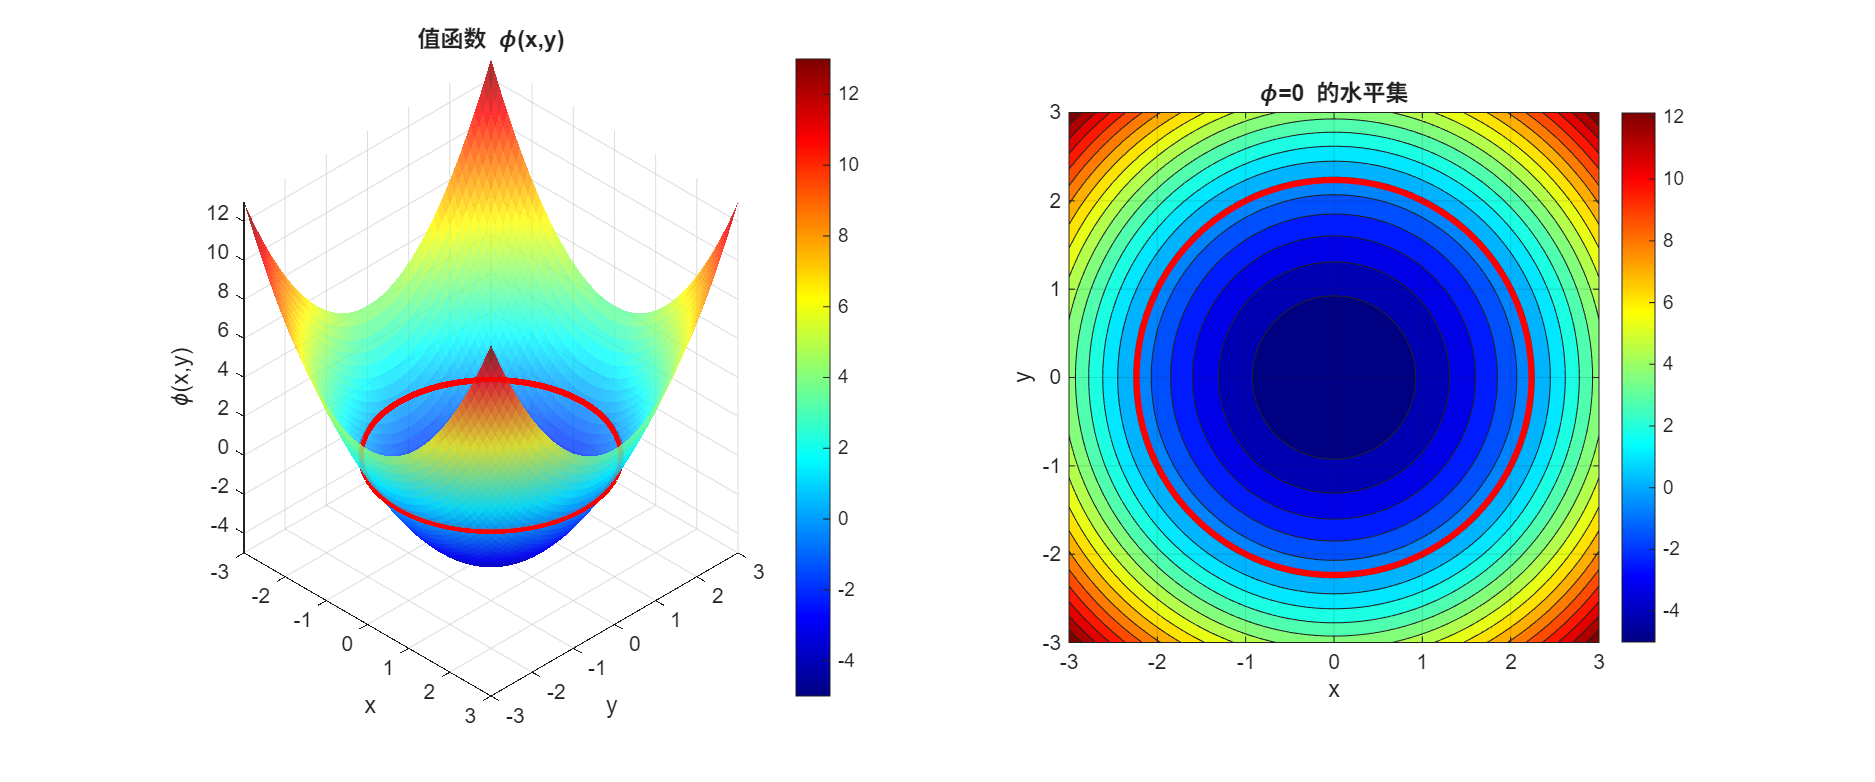
\includegraphics[width=0.8\textwidth]{figures/levelSetFunctionandTargetSet.png}
    \caption{水平集函数与目标集}
    \label{fig:levelSetFunctionandTargetSet}
\end{figure}

如图 \ref{fig:levelSetFunctionandReachableSet} 所示，在 $t (t<0)$ 时刻， $\phi<0$  的区域则对应于后向可达集 $\mathcal{R}_t(\mathcal{T})$ 的内部，即那些具备在未来 $t=0$ 时到达目标集潜力的状态集合。
\vspace{1.5ex}
\begin{figure}[htbp]
    \centering
    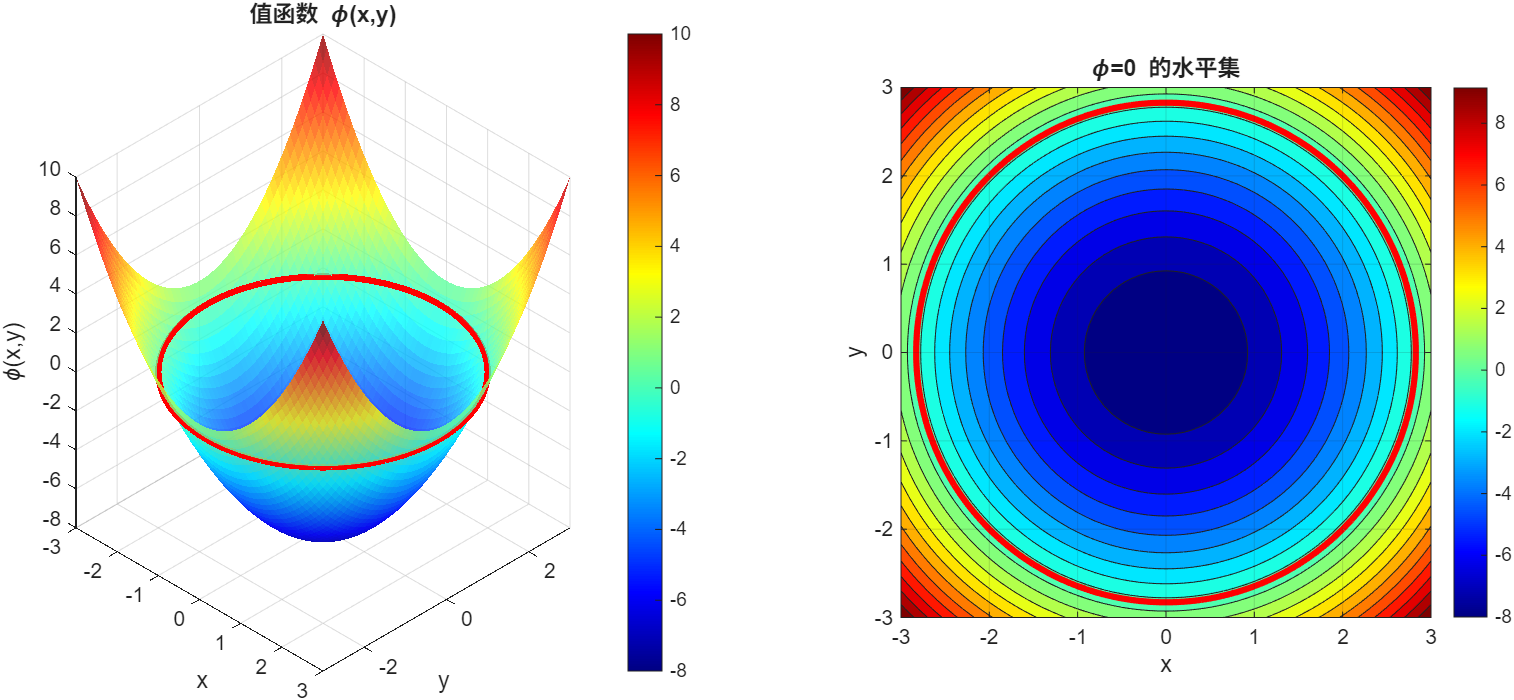
\includegraphics[width=0.7\textwidth]{figures/levelSetFunctionandReachableSet.png}
    \caption{水平集函数与后向可达集}
    \label{fig:levelSetFunctionandReachableSet}
\end{figure}



需要特别强调，$\phi(\mathbf{x},t)<0$ \textbf{并不等价于}“系统此刻在目标集内”，其表示一种\emph{可达性语义}——仅说明该状态具备在未来到达目标集的潜力，而非当前已处于目标集。





%% 第三节
\section{后向可达集与最优化控制的联系}
\subsection{问题的等价重述}
根据第二节的定义，后向可达集的核心语义是：
\begin{center}
	\fbox{\textbf{存在控制可以使得某状态最终进入目标集合的所有状态的集合}。}
\end{center}

这是一类\emph{存在性问题}，而非性能最优问题。然而，该存在性问题可以通过一个最优化值函数来等价刻画。

为此，我们首先用一个水平集函数 $\ell : \mathbb{R}^n \to \mathbb{R}$ 描述目标集：

\[
\ell(\mathbf{z}) \le 0 
\quad \Longleftrightarrow \quad 
\mathbf{z} \in \mathcal{T}.
\]
例如，$\ell$ 可以取为目标集的 signed distance function 或其连续近似。

\subsection{值函数的构造}
对于任意 $(\mathbf{x},t)$，定义如下值函数：

\begin{equation}
V(\mathbf{x},t)
:=
\inf_{\mathbf{u}(\cdot) \in \mathcal{U}^{[t,0]}}
\;
\min_{\tau \in [t,0]}
\;
\ell\!\big(
\mathbf{x}^{\mathbf{u}}_{\mathbf{x},t}(\tau)
\big).
\end{equation}


其中：
\begin{itemize}
    \item $\mathbf{x}^{\mathbf{u}}_{\mathbf{x},t}(\tau)$ 为从 $(\mathbf{x},t)$ 出发、在控制 $\mathbf{u}(\cdot)$ 下产生的状态轨迹；
    \item 内层 $\min_{\tau \in [t,0]}$ 表示该轨迹在时间区间内所达到的最小 $\ell$ 值；
    \item 外层 $\inf$ 表示在所有可行控制中选择使该最小值尽可能小的控制策略。
\end{itemize}

注意，这里的“最小化”并不是为了获得某种性能指标，而是为了刻画以下逻辑等价关系。

\begin{defn}{上、下确界}{inf & sup}
设 $S$ 是实数集合，若存在实数 $m$ 满足以下两个条件：
\begin{itemize}
    \item 对任意 $s \in S$，恒有 $s \ge m$；
    \item 对任意 $\epsilon > 0$，存在 $s' \in S$ 使得 $s' < m + \epsilon$。
\end{itemize}
则称 $m$ 是集合 $S$ 的下确界，记为 $\inf S$。

同样地，若存在实数 $M$ 满足以下两个条件：
\begin{itemize}
    \item 对任意 $s \in S$，恒有 $s \le M$；
    \item 对任意 $\epsilon > 0$，存在 $s' \in S$ 使得 $s' > M - \epsilon$。
\end{itemize}
则称 $M$ 是集合 $S$ 的上确界，记为 $\sup S$。
\end{defn}
\subsection{存在性与值函数符号的等价}

我们现在说明：

\[
V(\mathbf{x},t) \le 0
\quad \Longleftrightarrow \quad
\mathbf{x} \in \mathcal{R}_t(\mathcal{T}).
\]

证明思路如下：

\paragraph{(1) 若 $V(\mathbf{x},t) \le 0$}

根据定义，存在控制 $\mathbf{u}(\cdot)$ 使得

\[
\min_{\tau \in [t,0]} 
\ell\big(
\mathbf{x}^{\mathbf{u}}_{\mathbf{x},t}(\tau)
\big)
\le 0.
\]

因此，存在某个时刻 $\tau^\ast \in [t,0]$ 使得

\[
\ell\big(
\mathbf{x}^{\mathbf{u}}_{\mathbf{x},t}(\tau^\ast)
\big)
\le 0,
\]

即轨迹在该时刻进入目标集。

特别地，当问题定义为“在时刻 $0$ 到达目标集”时，上述条件可进一步收缩为

\[
\ell\big(
\mathbf{x}^{\mathbf{u}}_{\mathbf{x},t}(0)
\big)
\le 0,
\]

从而 $(\mathbf{x},t)$ 属于后向可达集。

\paragraph{(2) 若 $\mathbf{x} \in \mathcal{R}_t(\mathcal{T})$}

根据后向可达集定义，存在控制使得

\[
\mathbf{x}^{\mathbf{u}}_{\mathbf{x},t}(0) \in \mathcal{T},
\]

即

\[
\ell\big(
\mathbf{x}^{\mathbf{u}}_{\mathbf{x},t}(0)
\big)
\le 0.
\]

因此

\[
\min_{\tau \in [t,0]}
\ell\big(
\mathbf{x}^{\mathbf{u}}_{\mathbf{x},t}(\tau)
\big)
\le 0,
\]

进而 $V(\mathbf{x},t) \le 0$。

\subsection{与水平集函数 $\phi$ 的一致性}

令 $\phi(\mathbf{x},t)$ 为满足

\[
\phi(\mathbf{x},t) \le 0
\quad \Longleftrightarrow \quad
\mathbf{x} \in \mathcal{R}_t(\mathcal{T})
\]

的隐式函数。

在向量场满足 Lipschitz 连续、控制集紧致且不存在外部扰动的条件下，可以证明：

\[
V(\mathbf{x},t) \equiv \phi(\mathbf{x},t).
\]

因此，后向可达集的计算可以通过求解该值函数完成，而该值函数满足一个 Hamilton---Jacobi 型偏微分方程。

\subsection{本节小结}

我们得到一个重要结论：

\begin{center}
\fbox{
后向可达集问题虽然是存在性问题，
但可以等价地转化为一个最优化值函数问题。
}
\end{center}

这里的“最小化”并非性能优化意义上的最优控制，
而是对“存在可行控制”的一种数值刻画方式。

接下来，我们将基于动态规划原理，推导该值函数所满足的 Hamilton---Jacobi 方程。

\vspace{5ex}

%% 第四节
\section{推导Hamilton---Jacobi 方程}
后向可达集的边界演化并非无迹可寻。通过动态规划原理（Dynamic Programming Principle, DPP），我们可以
将一个跨越整个时间域 $[t,0]$ 的存在性问题，转化为一个在时空邻域内求解偏微分方程的局部问题。
\subsection{动态规划原理与递归关系}

后向可达集 $\mathcal{R}_t(\mathcal{T})$ 的边界可以看作一个波前(front)，它从目标集 $\mathcal{T}$ (t=0时刻)
开始，向着过去(t<0)的方向传播。这个波前的传播速度和方向并不是均匀的，而是取决于，在当前边界点 $\mathbf{x}$，
是否存在某种控制 $\mathbf{u}$ 能够让该状态更有利于保持或进入目标集（即让值函数 $\phi$ 继续减小或保持 $\le$ 0）。

正是这种“最有利方向”的局部决策，决定了整个可达集边界的演化规律，而DPP是将全局最优决策拆解
为局部决策的数学工具。

\subsection{值函数沿最有利方向的瞬时变化率（物理直觉）}

考虑值函数 $\phi(\mathbf{x},t)$ （或等价的 $V(\mathbf{x},t)$），其水平集 $\phi = 0$ 就是后向可达集的边界。
在某个状态 $\mathbf{x}$ 处，梯度 $\mathbf{p} = \nabla \phi (\mathbf{x},t)$ 指向 $\phi$ 增长最快的方向（法线外），
因此 $-\mathbf{p}$ 指向 $\phi$ 下降最快的方向（法线内）。

系统若沿着动力学 $\dot{\mathbf{x}} = f(\mathbf{x},\mathbf{u})$ 运动一小段时间 $\Delta t$，则值函数的变化率可以近似表示为：
\begin{equation}
    \dot{\phi} \approx \nabla \phi \cdot f(\mathbf{x},\mathbf{u}) = \mathbf{p}^\top f(\mathbf{x},\mathbf{u})
\end{equation}

为了能让状态尽可能“保持在可达集内”或“向可达集内部演进”，我们希望 $\dot{\phi}$ 尽可能小（最好 < 0）。因此，在所有容许控制中，
我们关心的是：
\begin{equation}
    \boxed{
        H^*(\mathbf{x},\mathbf{p}) = \min_{\mathbf{u} \in \mathcal{U}} \ \mathbf{p}^\top f(\mathbf{x},\mathbf{u})
    }
\end{equation}
\begin{itemize}
 \item 若 $H^*(\mathbf{x},\mathbf{p}) < 0$，说明\textbf{存在}控制使值函数下降，边界可以继续向后（向过去）扩张；
 \item 若 $H^*(\mathbf{x},\mathbf{p}) \ge 0$，说明所有控制都无法让值函数下降，边界在此处“冻结”或停止扩张。
\end{itemize}

下面我们定义Hamiltonian函数
\begin{equation}\label{eq:Hamiltonian}
    H^*(\mathbf{x},\mathbf{p}):=\inf_{\mathbf{u}\in\mathcal U}\ \mathbf{p}^\top f(\mathbf{x},\mathbf{u})
\end{equation}

式中，$\mathbf{p}$ 是一个与状态空间维度相同的向量，通常被称为\textbf{协态}或\textbf{成本ate}，在后续分析中将被赋予特定的物理与语义含义。
\begin{defn}{Hamiltonian函数}{Hamiltonian}
设 $f:\mathbb{R}^n \times \mathbb{R}^m \to \mathbb{R}^n$ 是一个向量场，$\mathcal{U} \subset \mathbb{R}^m$ 是一个控制输入集合，$\mathbf{p} \in \mathbb{R}^n$ 是一个协态向量，则定义Hamiltonian函数 $H^*:\mathbb{R}^n \times \mathbb{R}^n \to \mathbb{R}$ 为
\[
H^*(\mathbf{x},\mathbf{p}) := \inf_{\mathbf{u} \in \mathcal{U}} \mathbf{p}^\top f(\mathbf{x},\mathbf{u})
\]
其中，$\mathbf{p} = \frac{\partial V}{\partial \mathbf{x}}$，$\mathbf{p}^\top f(\mathbf{x},\mathbf{u})$ 表示向量 $\mathbf{p}$ 与 $f(\mathbf{x},\mathbf{u})$ 的内积。
\end{defn}
这正是 Hamiltonian 中取 \textbf{极小值} 的核心语义来源：它对应“是否存在使可达性改善的控制”。


\subsection{DPP与离散时间递推关系}
现在我们从DPP的角度来看这一思想。

对于任意满足$t \le 0$ 的 $(\mathbf{x},t)$， 不考虑外界扰动, 定义值函数如下
\begin{equation}\label{eq:valueEqu}
    V(\mathbf{x},t):=\inf_{\mathbf{u}(\cdot)}\ \min_{\tau\in[t,0]}\ \ell\big(\mathbf{x}^{\mathbf{u}}_{\mathbf{x},t}(\tau)\big)
\end{equation}

%其中，  $\mathbf{x}^{\mathbf{u}}_{\mathbf{x},t}(\cdot)$ 代表系统在$t$时刻从
%状态$\mathbf{x}$出发，在控制输入$\mathbf{u}(\cdot)$作用下的状态轨迹。$\ell(\mathbf{x})$ 代表的是 $\phi(\mathbf{x},0)$，也即 $t=0$ 的隐式值函数。
%$\inf$ 代表的是
%最小值的上界，也叫做下确界。


对于任意固定的控制信号 $\mathbf{u}(\cdot)$ 和任意的 $\Delta t>0$，以下恒等式成立\cite{ref1}：
\begin{equation}\label{eq:splitMin}
    \min_{\tau\in[t,0]} \ell(\mathbf{x}(\tau))
    =
    \min\Big(\ell(\mathbf{x}(t)),\ \min_{\tau\in[t+\Delta t,0]} \ell(\mathbf{x}(\tau))\Big)
\end{equation}

式 \ref{eq:splitMin} 的物理含义是，\textbf{当前以及未来的最小值，是当前值和未来最小值的较小者}。这其实就是动态规划的离散形式。


进一步，选取所有控制信号可以得到的 $\min_{\tau\in[t,0]}$ 的下确界 $\inf_{\mathbf{u(\cdot)}}  \min_{\tau\in[t,0]} \ell(\mathbf{x}(\tau))$，
即 $V(\mathbf{x},t)$，满足如下动态规划递归关系：
\begin{equation}\label{eq:DPP}
    V(\mathbf{x},t)
    =
    \inf_{\mathbf{u}\in\mathcal U}\ 
    \min\Big(\ell(\mathbf{x}),\ V(\mathbf{x}(t+\Delta t),t+\Delta t)\Big)  
\end{equation}
 
式 \ref{eq:DPP} 中，$\mathbf{x}(t+\Delta t)$ 是从 $(\mathbf{x},t)$ 出发，
在 $[t,t+\Delta t]$ 上施加恒定控制 $\mathbf{u}$ 后达到的状态。

\subsection{从离散到连续：无穷小极限与两种演化模式}
假设 $V$ 在 $(\mathbf{x},t)$ 可微， 那么以下的一阶泰勒展开成立
\begin{equation}\label{eq:taylor}
    V(\mathbf{x}(t+\Delta t),t+\Delta t)
    =
    V(\mathbf{x},t)
    +\Delta t\Big(\partial_t V(\mathbf{x},t)+\nabla V(\mathbf{x},t)^\top f(\mathbf{x},\mathbf{u})\Big)
    +o(\Delta t)
\end{equation}

对于非线性动力学系统式 \ref{eq:dyn}， 有
\begin{equation}\label{eq:flow}
    \mathbf{x}(t+\Delta t)=\mathbf{x}+f(\mathbf{x},\mathbf{u})\Delta t+o(\Delta t)  
\end{equation}

将式 \ref{eq:taylor} 代入 式 \ref{eq:DPP} 中， 可以得到
\begin{equation}\label{eq:substitute}
    V(\mathbf{x},t)
    =
    \inf_{\mathbf{u}\in\mathcal U}\ 
    \min\Big(\ell(\mathbf{x}),\ V(\mathbf{x},t)+\Delta t(\partial_t V+\nabla V^\top f(\mathbf{x},\mathbf{u}))+o(\Delta t)\Big)
\end{equation}


\emph{情况 1 (未冻结):}当式 \ref{eq:DPP} 的 $\min(\cdot, \cdot)$ 内部的第二项严格小于第一项，
那么 $\min$ 选择第二项，那么式 \ref{eq:substitute} 可以被简化为

\begin{equation}\label{eq:unfrozen}
    0
    =
    \inf_{\mathbf{u}\in\mathcal U}\ 
    \Big(\partial_t V+\nabla V^\top f(\mathbf{x},\mathbf{u})\Big)
\end{equation}

将式 \ref{eq:Hamiltonian} 代入式 \ref{eq:unfrozen} 中， 可以得到
\begin{equation}\label{eq:unfrozenHamiltonian}
    \partial_t V + H^*(\mathbf{x},\mathbf{p}) = 0
\end{equation}


\emph{情况 2 (冻结):}当式 \ref{eq:DPP} 的 $\min(\cdot, \cdot)$ 内部的第一项小于等于第二项，
那么 $\min$ 选择第一项，那么式 \ref{eq:substitute} 可以被简化为
\begin{equation}\label{eq:frozen}
    V(\mathbf{x},t) = \ell(\mathbf{x})
\end{equation}

这意味，一旦系统状态进入了局部最小值，将停止向后的演进。这是由 $\min_{\tau \in [t,0]}$所决定的。
也即
\begin{equation}\label{eq:frozenHamiltonian}
    \partial_t V(\mathbf{x},t) = 0
\end{equation}
\subsection{HJ 方程的最终形式}
将式 \ref{eq:frozenHamiltonian} 和式 \ref{eq:unfrozenHamiltonian} 联合，可以得到
\begin{equation}\label{eq:HJ}
    \partial_t V + \min\{0, H^*(\mathbf{x},\mathbf{p})\} = 0
\end{equation}

其终端条件为
\begin{equation}\label{eq:terminalCondition}
    V(\mathbf{x},0) = \ell(\mathbf{x})
\end{equation}

至此，式 \ref{eq:terminalCondition} 我们发现后向可达集的计算本质上就是一个最优化求解问题，求解 $\mathbf{u}$ 使得值函数 $V(\mathbf{x},t)$最小。

\subsection{本节小结}

\begin{itemize}
\item $H^* < 0$：存在控制使 $\phi$ 下降 $\quad \Rightarrow$ 可达集边界继续向 $t<0$ 扩张
\item $H^* \ge 0$：所有控制都无法使 $\phi$ 下降 $\quad \Rightarrow$ 边界在此“冻结”
\item $\min\{0, H^*\}$ 正是为了在“还能扩张”和“已达极限”两种情况之间自动切换
\item 时间反向积分是因为我们在从已知的目标（t=0）反推未知的初始状态集
\end{itemize}

\section{常见困惑与澄清}

\subsection{为什么Hamiltonian要计算u引起的极小值}
基于上述值函数一阶变化率的分析，我们定义了后向可达集分析中的核心算子——Hamiltonian函数，其表达式为：
\[
H(\mathbf{x},\mathbf{u}) = \min_{\mathbf{u} \in \mathcal{U}} \mathbf{p}^\top f(\mathbf{x},\mathbf{u})
\]
在一些情况下，$\min$ 也会被写成 $\inf$，但其核心语义并未改变。

注意，\textbf{这里的极小值运算 $\min$ 并不是性能优化意义下的最优求解，而是对于可达性存在性的刻画。}

让我们再来捋一遍。

我们希望的是存在一个控制能让值函数减小，也就是 $H(\mathbf{x},\mathbf{p}) < 0$，而 $\mathbf{p}$ 是控制 $\mathbf{u}$
的函数。

在这么多的可选控制里，我们只要找到能让 $\mathbf{p}^\top f(x,u)$ 最小的那个控制，就能判断是否存在一个控制能让值函数下降。因此，这里
的极小值运算 $\min$ 对应的逻辑量词是存在量词 $\exists$，而其运算空间是控制空间 $\mathcal{U}$，而非状态空间 $\mathbb{R}^n$。

如果我们用$\max$ 来定义 Hamiltonian,也即
\[
H(\mathbf{x},\mathbf{u}) = \max_{\mathbf{u} \in \mathcal{U}} \mathbf{p}^\top f(\mathbf{x},\mathbf{u})
\]

那么就会对应全称量词 $\forall$，也就是我们能要求任何的控制都可以让系统状态进入目标集，这显然不符合我们前面对于可达性的语义需求。

如果读者感兴趣，可以去自己看下王爽的论文 \cite{ref2}，他的问题定义决定了他最后的Hamiltonian是 $\max$，而不是 $\min$。
\subsection{为什么会出现外层的$\min(0,H)$}

我们前面已经推导过，后向可达集的HJ方程的最终形式为：
\begin{equation*}
    \partial_t V + \min\{0, H^*(\mathbf{x},\mathbf{p})\} = 0
\end{equation*}

关于上面这是式子里的 $\min(0,H)$ 我们回忆这个式子怎么来的，是式 \ref{eq:unfrozenHamiltonian} 和式 \ref{eq:frozenHamiltonian} 两种情况的联合。
而这两者是由式 \ref{eq:DPP} 中 $\min(\ell(\mathbf{x}), V(\mathbf{x}(t+\Delta t),t+\Delta t))$ 的两种情况决定的。

这两种情况又是由 $\min_{\tau \in [t,0]}$ 的定义决定的。
因此，$\min(0,H)$ 的存在是为了在“还能扩张”和“已达极限”两种情况之间自动切换。
它的物理意义是：当 $H < 0$ 时，边界可以继续向后扩张；当 $H \ge 0$ 时，边界在此处“冻结”，无法再向后扩张了。

换句话说，我们因此求得的可达集，只要这个状态点在 $\tau \in [t,0]$ 内曾经进入过目标集，那么它就属于可达集；如果这个状态点在 $\tau \in [t,0]$ 内从未进入过目标集，那么它就不属于可达集。

如果我们求得是终端可达集，也就是严格要求在 $\tau=0$ 时刻进入目标集，那么式 \ref{eq:valueEqu} 中的 $\min_{\tau \in [t,0]}$ 就不存在了。故而也就不需要 $\min(0,H)$ 了，直接 $H$ 就可以了。
也就是
\begin{equation*}
    \partial_t V + H^*(\mathbf{x},\mathbf{p}) = 0   
\end{equation*}



\subsection{为什么时间反向}
在后向可达集分析中，所谓“时间反向”并不意味着物理上的时间倒流或反向演化。实际上，后向可达集问题的求解过程并不涉及任何形式的时间反转。对于一个给定的初始状态 \(\mathbf{x}\)，我们是正向地去计算值函数 \(V(\mathbf{x}, \tau)\)，并通过最小化值函数来分析系统的可达性。

具体而言，值函数 \(V(\mathbf{x}, \tau)\) 描述了从状态 \(\mathbf{x}\) 开始，在控制输入作用下，系统能否在未来时间内到达目标集。
如果我们定义的时间区间是 $\tau \in [T,0]$， 那么值函数 \(V(\mathbf{x}, T)\) 在时刻 \(T\) 与目标集的水平集函数 \(\ell(\mathbf{x})\) 相等，即：
\[
V(\mathbf{x}, T) = \ell(\mathbf{x}),
\]
% 表示状态 \(\mathbf{x}\) 恰好处于目标集的边界。

因此，在这个过程中，虽然在一些文献中使用“时间反向”这一表述，但实际上我们是在正向计算值函数并判断是否能够通过某种控制策略使得系统从给定的初始状态进入目标集。这一过程并不涉及物理时间的倒流，而是通过优化计算最优控制策略，确保系统能够进入目标集。
\section{总结}
本文从研究者的视角，对后向可达集的核心概念、数学定义及Hamilton---Jacobi方程的关键细节进行了系统性梳理，针对学习过程中易困惑的时间方向、Hamiltonian极值运算、值函数语义等问题给出了明确的解释，核心观点可概括为三点：
\begin{itemize}
    \item 后向可达集解决的是\textbf{控制策略的存在性问题}，而非控制律的设计问题，这是其与最优控制等问题的本质区别；
    \item Hamiltonian 中的极小值运算``$\min$''并非性能优化，而是对可达性存在性的数学表达，其运算空间为控制空间；
    \item 值函数 $V$ 的时间演化，刻画的是\textbf{可达性边界的扩张}，而非系统的实际物理运动，不涉及时间倒流。
\end{itemize}

上述核心理解为后向可达集在飞行器安全分析、失效后能力评估、鲁棒控制等实际工程问题中的应用奠定了概念基础，也是后续开展BRS数值求解、工程应用的前提。

关于可达集的计算，可以使用 Ian Mitchell 教授的 Level Set Toolbox（MATLAB，\url{https://www.cs.ubc.ca/~mitchell/ToolboxLS}）或
Stanford ASL 团队维护的 helperOC（MATLAB 包装器，\url{https://github.com/HJReachability/helperOC}）以及
hj\_reachability（Python/JAX 版本，\url{https://github.com/StanfordASL/hj_reachability}）等工具箱进行数值求解。感兴趣的读者
可以尝试自己使用，后续笔者也会详细介绍这些工具箱的使用方法。

最后，送给读者一句话：

\vspace{3ex}

\noindent
\fbox{%
    \parbox{0.97\textwidth}{
        \begin{quote}
        \vspace{4ex}
        It might be well for all of us to remember that, while dif\mbox{}fering widely in the various little bits we know, in our finite ignorance we are all equal.
        \vspace{2ex}
        \\
        我们不妨都记住这一点：虽然我们在各自所知的细枝末节上差异很大，但在我们有限的无知面前，我们都是平等的。
        \begin{flushright}
        ---Karl Popper, \emph{Conjectures and Refutations}
        \end{flushright}
        \end{quote}
    }
}


%\textbf{The Safe Autonomous Systems Lab} 

%\subsection{Available Toolboxes}
%\begin{itemize}
%	\item helperOC (MATLAB) https://github.com/HJReachability/helperOC . this is essentially 
%	a user-friendly wrapper with extra functionality for Prof. Ian Mitchel’s level set toolbox.
%    \item hj\_reachability (Python) https://github.com/StanfordASL/hj\_reachability. This is the python implementation of the above toolboxes, 
%    lead by Edward Schmerling at Stanford.  It is much more efficient than the MATLAB version 
%    and has an active group maintaining and updating it.  It currently lacks some of the niche 
%    functionality of the helperOC toolbox, but is very good for most standard reachability 
%    applications and is adding new functionality rapidly.
%end{itemize}

\begin{thebibliography}{5}  

\bibitem{ref1}K.Cong, D.Ma, Longitudinal dynamic envelope solution and transition path optimization based on reachability analysis for fixed-wing VTOL UAVs, Aerospace Science and Technology, 2024
\bibitem{ref2}王爽,詹浩. 飞行最大可控边界集及其机动边界保护控制[J]. 西北工业大学学报.[C].2014,32(4).
%\bibitem{ref3}田晓曦,刘振鹏,彭宝权. 地方高校开展教育人工智能深度融合的路径探究[A]. 中共沈阳市委、沈阳市人民政府.第十七届沈阳科学学术年会论文集[C].中共沈阳市委、沈阳市人民政府:沈阳市科学技术协会,2020:5.
%\bibitem{ref4}柏卓君,潘勇,李仲余.彩色多普勒超声在早期胚胎停育诊断中的应用[J].影像研究与医学应用,2020,4(18):129-131.
%\bibitem{ref5}杨芸.我院2018年人血白蛋白临床应用调查与分析[J].上海医药,2020,41(17):34-35+74.

\end{thebibliography}

\end{document}